\documentclass[12pt]{article}
\usepackage[utf8]{inputenc}
\usepackage[brazil]{babel}
\usepackage{hyphenat}
\usepackage{graphicx}
\usepackage{amsmath}
\graphicspath{{images/}}

% ---- Capa
\title{%
    Modelagem de Sistemas Dinâmicos\\ % \\ pula linha
    \large Relatório Trabalho 2}
\author{Erica da Cunha Ferreira \\Raiane Borges}
\date{Novembro 2020}
\begin{document}
\maketitle

%-----Sumário
\newpage
\tableofcontents

%----Pág 1
\newpage
\section{Resumo} % \quad = Tab
\quad O trabalho tem como objetivo modelar teoricamente e analisar um motor de corrente continua (DC) controlado por corrente de armadura e  comparar os resultados da modelagem teórica e experimental.

\section{Introdução}

\quad  Neste trabalho é analisado o motor de corrente continua (DC) controlado por corrente de armadura com a entrada de tensão $V_a (t)(V)$ e com saídas de posição angular $\theta_m (t)$ e velocidade angular $\omega_m (t)(rad/s)$ representado pela Figura 1.

\begin{figure}[h] %h é para here - aqui
    \centering
    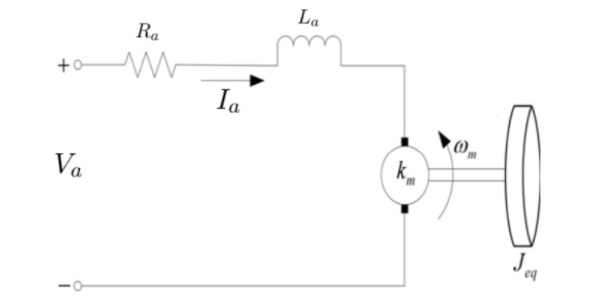
\includegraphics[width = 0.7\textwidth]{Sistema.jpg}
    \caption{Modelo esquemático do motor de corrente continua (DC)}
    \label{fig:mesh1}
\end{figure}

\quad Tendo este sistema as seguintes característcas fornecidas pelo fabricante:

\begin{itemize}
    \item Resistência da armadura, $R_a = 10.6 \Omega$
    \item Indutância da armadura, $L_a$ = 0.82 $mH$
    \item Momento de Inércia do Rotor do Motor, $J_m = 1.16 10^-6$ 
    \item Constantes do Motor, $K_m = K_e = K_t =$ 0.0502 $Nm/A$
    \item Tensão Máxima, 15 volts
    \item Massa do disco de inércia, 0.068 $kg$
    \item Raio do disco de inércia, 0.0248 $m$
\end{itemize}

\section{Modelagem Teórica}
\subsection{Diagrama de Blocos}

\quad A partir da análise do circuito e do uso do softwares Matlab e Simulink, pode ser construído o diagrama de blocos abaixo, é importante salientar, que o atrito do sistema foi desconsiderado.

\begin{figure}[h] 
    \centering
    \includegraphics[width=0.9\textwidth]{Diagrama de Bloco.jpg}
    \caption{Diagrama de Blocos do sistema}
    \label{fig:mesh2}
\end{figure}

\quad Pelo circuito representado pelo diagrama de blocos, as seguintes equações são deduzidas.\\
\quad \\Equações:

\begin{equation}
    V_a (s) = I_a(s) \cdot R_a + s\cdot L_a(s)\cdot I_a (s) + K_e\cdot \omega_m (s)
\end{equation}

\begin{equation}
    J_m\cdot s \cdot \omega_m (s) = K_t \cdot I_a (s)
\end{equation}

\begin{equation}
    T_m = K_t \cdot I_a (s)
\end{equation}

\begin{equation}
    E_b = K_e \cdot \omega_m (s)
\end{equation}

\subsection{Função de Transferência}

\begin{equation}
    G(s) = \frac{\omega_m (s)}{V_a (s)} = \frac{K_t}{J_m \cdot s \cdot (s \cdot L_a + R_a) + K_t \cdot K_e}
\end{equation}

\subsection{Sistema de Espaço de Estados}
\begin{equation}
    \dot{x} = 
    \begin{bmatrix} 
        \frac{-R_a}{L_a} & \frac{-K_e}{L_a} \\
        \frac{K_m}{J_m} & 0
    \end{bmatrix}
    \begin{bmatrix}
        i_a\\
        \omega_m
    \end{bmatrix}
    +
    \begin{bmatrix}
        \frac{1}{L_a}\\
        0
    \end{bmatrix}V_a
\end{equation}


\section{Identificação Experimental}
\section{Validação dos Modelos}
\section{Discussão}
\section{Conclusão}

\end{document}
